\chapter{Occupant-Oriented Room-Level Zoning}

Our approach consists of using empirical models that are learned using
historical and real-time data to strategically control the delivery of heated or
cooled air to locations where comfort is needed the most. An assessment of room
occupancy is used to decide which rooms have to be conditioned, a profile of the
thermal characteristics of the house will help decide which non-occupied rooms
have to be conditioned in order to maximize the benefit on occupied rooms, and
the operating characteristics of the HVAC system will help schedule heating and
cooling stages that minimize energy expenditure. The zone controller utilizes
this information to efficiently heat or cool the house in order to minimize
energy waste while not compromising on occupant comfort. We use X10 and PIR
motion sensors to build the room occupancy model; a airflow meter to build a
thermal flow model for the house; and temperature sensors to monitor temperature
changes in rooms.

\begin{figure}[t]
  \centering    
  \subfigure[Traditional Zoning]{
  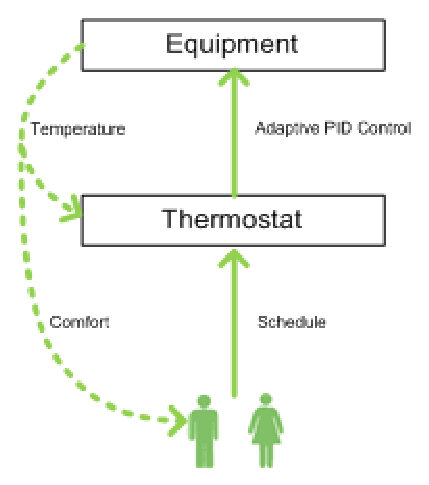
\includegraphics[width=0.25\columnwidth]{fig/zone1}
  \label{fig:zone1}
  }
  \hspace{0.25in}
  \subfigure[Occupancy-Oriented Room-Level Zoning]{
  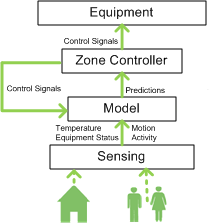
\includegraphics[width=0.25\columnwidth]{fig/sub-zoning}
  \label{fig:overview}
}
  \caption{Traditional Zoning vs. Occupancy Oriented Room-Level Zoning.}
  \label{fig:systemOverview}
\end{figure}

Conventional approaches to HVAC zoning use thermostatic control of the
equipment, as illustrated in Figure~\ref{fig:zone1}: residents provide a
schedule to the thermostat, which controls the equipment. For instance, the
thermostat could be scheduled to condition only the top floor, where the
bedrooms are located, from 11:00 PM to 8:00 AM and condition only the bottom
floor, where the living areas are located, from 8:00 AM to 11:00 PM. The most
advanced thermostats use adaptive PID controllers to condition each zone. These
controllers learn control parameters over time but do not dynamically change
zones based on occupancy. 

Manual thermostats cannot optimally control a room-level zoned centralized HVAC
system due to its complexity. Our approach to controlling such a system is
illustrated in Figure~\ref{fig:systemOverview}. Building parameters such as
temperature and the status of HVAC equipment are monitored along with occupant
motion using a sensing subsystem comprised of cheap, off-the-shelf sensors. This
data is used to assess room occupancy, build a thermal flow model, and equipment
operation model. This information is used by the zone controller in order to
efficiently actuate the HVAC equipment and provide comfort to the occupants. 

\section{Intuition and Preliminary Studies}
Before implementing Smart Zone, we performed two simulation-based studies to
better understand whether, and why, such a system should be expected to save
energy. We also analyzed the occupancy data from a house to identify patterns in
room occupancy. We motivate this project through insights gained through this
analysis which are described in the following subsections.

\subsection{Effect of an Oversized HVAC System}
In houses with a typical non-zoned central heating and air conditioning system,
the size of the system is chosen based on the expected load of the entire
house. Therefore, using the same system to heat or cool only a fraction of the
house would mean that the system is oversized for the conditioned space. It is
well known that oversizing an HVAC system results in reduced efficiency of the
system. Our first study was designed to determine how much this oversizing would
reduce the potential for energy savings of a room-level zoning system.

\begin{figure}[t]
  \centering
  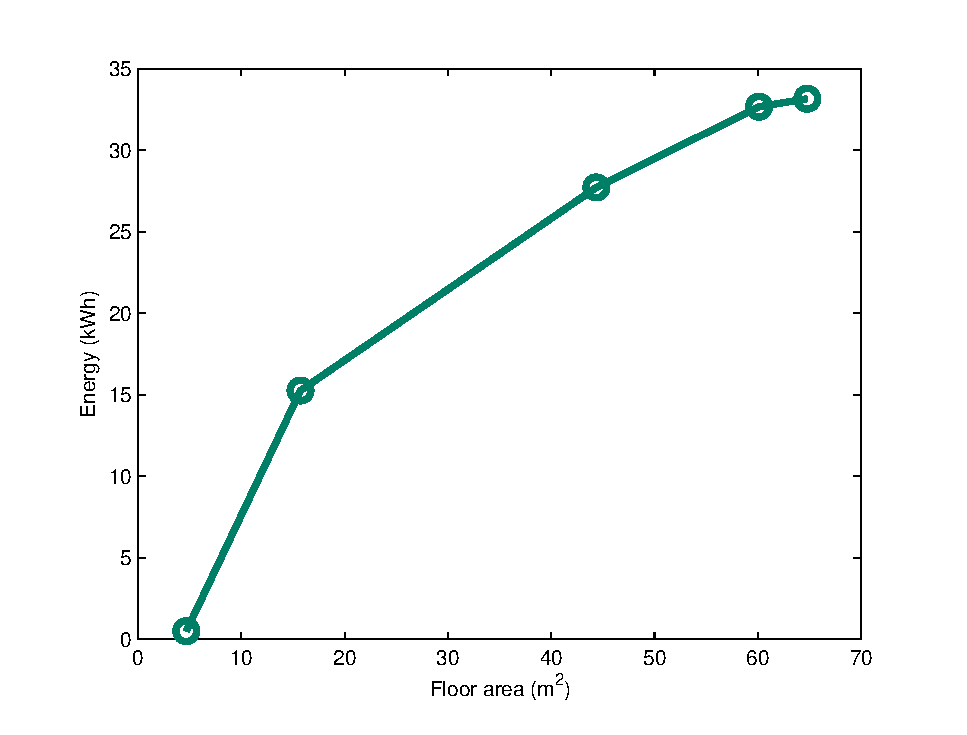
\includegraphics[width=0.6\columnwidth]{fig/areaVsEnergy}
  \caption[Effect of Floorspace on Energy Usage]{With an ideal system, the
    amount of energy used for conditioning a building is almost proportional to
    the floorspace being conditioned.}
  \label{fig:areaVsEnergy}
\end{figure}

We used the EnergyPlus building energy simulation
framework~\cite{crawley2004energyplus} to heat multiple buildings in simulation,
with increasing size from $5 \mathrm{m}^2$ to $65 \mathrm{m}^2$. The model
buildings had idealized insulation and leakage properties. All buildings were
heated with the same sized HVAC system, which was sized for a $65 \mathrm{m}^2$
building.  The results are shown in Figure~\ref{fig:areaVsEnergy}, which
indicate that the amount of energy required to heat a smaller building does
indeed decrease, even if the size of the HVAC system remains the same.  The
sub-linear curve indicates that some efficiency is lost for smaller buildings
due to the oversizing of the system.  However, this loss in efficiency does not
outweigh the gains from heating a smaller space.  From these results, we
postulate that room-level zoning can be effective, even when applied by
retrofitting a home with an existing HVAC system that was sized for the entire
house.


\subsection{Inter-room Leakage}
\label{subsec:interRoomLeakage}

Homes often have thin non-insulated walls and even doors between
adjacents rooms, which can reduce the effectiveness of room-level
zoning because of thermal leakage between rooms.  Our second study was
designed to explore how much this leakage would reduce the energy
savings of a room-level zoning system.  We used the EnergyPlus
simulation framework to heat a single room in a two-room building.  We
used five variations of the floor plan of the house, and the
conditioned room had a different number of exterior walls in each
variation.  The five variations are shown along the x-axis of
Figure~\ref{fig:wallsVsEnergyRoom}, and the energy required to heat
the shaded room for each floor plan is shown as a bar graph above each
variation.  These results indicate that the energy required to
condition a room is dramatically reduced as the number of exterior
walls of the room decreases.  In other words, a neighboring room is a
better thermal insulator than an exterior wall, even if the wall
between the conditioned room and the neighboring room is not
insulated.  This result indicates that leakage between conditioned and
unconditioned zones will not eliminate the energy-saving potential of
room-level zoning.

\begin{figure}[ht]
  \centering
  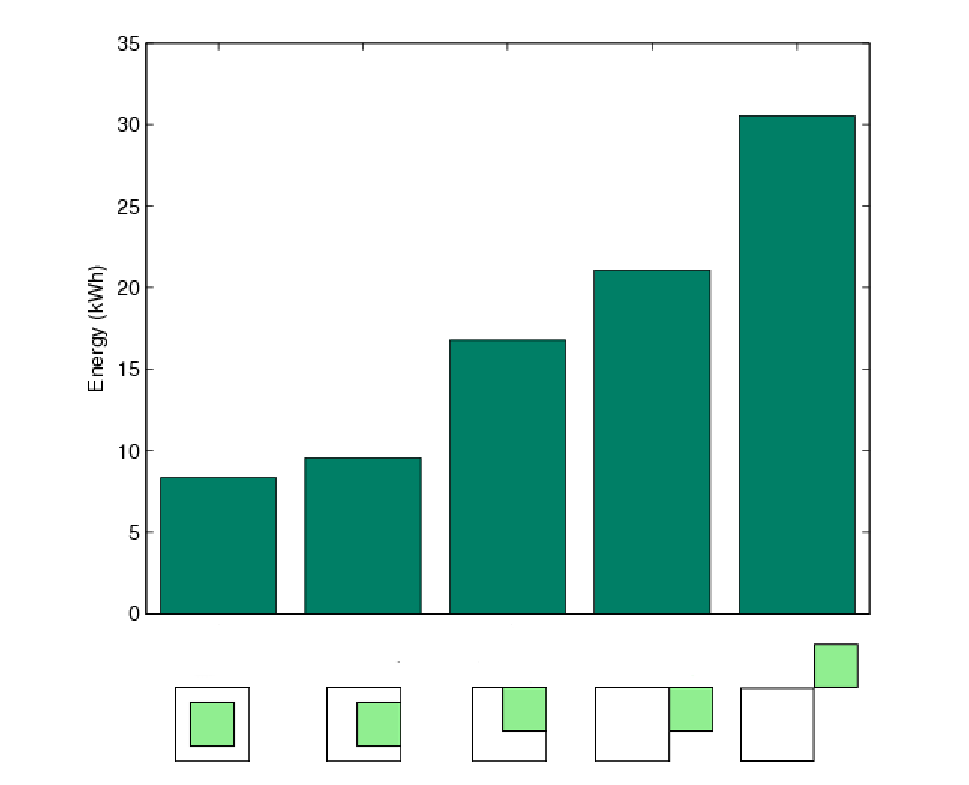
\includegraphics[width=0.55\columnwidth]{fig/wallsVsEnergyRoom}
  \caption[Effect of Exterior Walls on Energy Usage]{The energy required to
    condition a room decreases as its number of exterior walls is decreased.
    The x-axis depicts the position of the conditioned room (shaded) with
    respect to the unconditioned room (unshaded).}
  \label{fig:wallsVsEnergyRoom}
\end{figure}


\subsection{Room Occupancy}

Finally, our preliminary analysis showed that, even when a home is occupied, the
occupants use only a fraction of the house. For example, empirical analysis of
one home is shown in Figure~\ref{fig:roomUsage}, showing that primarily only one
room is used at night, three rooms are used in the evening, and four rooms are
used in the morning.

\begin{figure}[ht]
  \centering
%  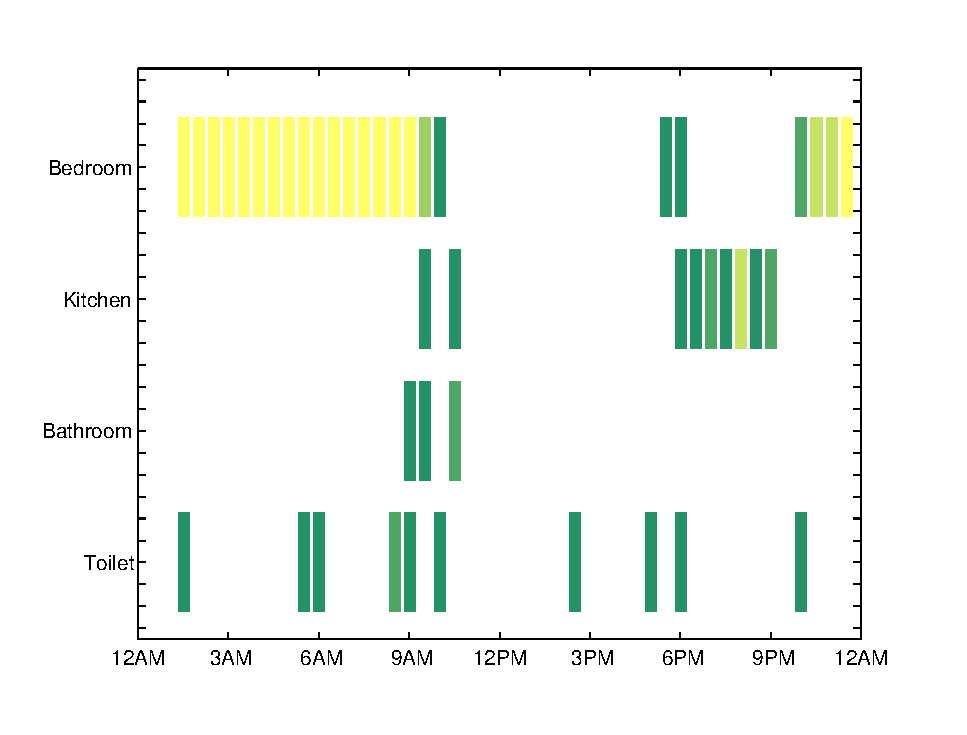
\includegraphics[width=0.6\textwidth]{fig/roomUsage}
  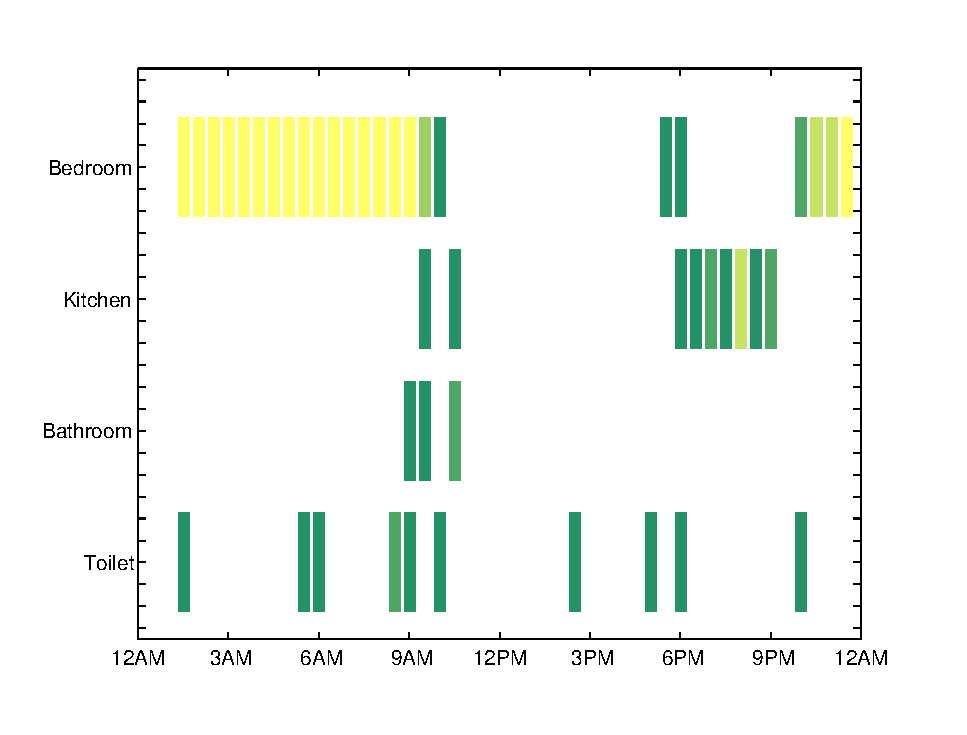
\includegraphics[width=1\columnwidth]{fig/roomUsage}
  \caption[Frequency of Room Usage Throughout a Day]{The frequency of room usage
    throughout a day changes. Darker colors indicate lower frequency while
    brighter colors indicate higher frequency usage with yellow being the
    highest frequency.}
  \label{fig:roomUsage}
\end{figure}
